\documentclass{article}

\title{Notes on shape calculus for fitted and nonfitted discretizations,  scrabbled down to be included in an eventual manuscript}
\author{Martin Berggren}
% Page sizes
\usepackage[pdftex,a4paper, height=230mm,width=164mm]{geometry} 
\usepackage[margin=15pt,font=small,labelsep=period,labelfont=sc]{caption} 
\usepackage[bf,compact,small,pagestyles]{titlesec}
%% Fonts
\usepackage{stix2}

\usepackage{tikz}
\usepackage{xcolor}

\usepackage{mathrsfs} % Fancy script fonts
\usepackage{microtype} % Better line breaks
\usepackage{mathtools}
\usepackage{amsthm}

% Thm styles
\newtheorem{theorem}{\textbf{Theorem}}[section]
\theoremstyle{remark}
\newtheorem{remark}[theorem]{\textit{Remark}}

% Amsmath option to number equations by section
\numberwithin{equation}{section}  


\usepackage{BOONDOX-ds} % Martin likes the Blackboard Bolds from these

% Math macros
\newcommand{\RR}{\mathbb{R}}
\let\bs\boldsymbol
\let\mb\mathbf

\usepackage{graphicx}

\begin{document}
\maketitle

\section{Optimization in $\RR^n$}\label{s:Rn}

As a background for the shape calculus carried out below, we shortly review and remark on related concepts in the context of ordinary gradient-based optimization.

%
Consider the unconstrained minimization problem in $\RR^n$,
\begin{equation}\label{e:unconRn}
\min_{x\in\RR^n} f(x).
\end{equation}
%
Typical iterative solvers of problem~\eqref{e:unconRn} constructs a consistent \textit{model function} around current iterate $x_n$, that is, functions $m_n$ satisfying
%
\begin{equation}
f(x_n + s) = f(x_n) + m_n(s) + o(\lvert s\rvert)\qquad\text{as $\lvert s\rvert\to0$.}
\end{equation}
%
For instance, both Newton’s method and the steepest-descent algorithm rely on a model function of the type
%
\begin{equation}\label{e:mndef}
m_n(s) = s\cdot g(x_n) + \frac12 s\cdot H(x_n) s.    
\end{equation}
%
The minimizer $s^*$ of $m_n$ is the solution of the linear system
%
\begin{equation}
H(x_n)s^* = - g(x_n). 
\end{equation}
%
Here, $g$ is the vector of partial derivatives of $f$ with components
%
\begin{equation}\label{e:gradient}
e_i\cdot g(x_n) = \frac{\partial f}{\partial x_i}(x_n) = 
%\lim_{t\to0}\frac{f(x_n + te_i)-f(x_n)}t = 
\frac d{dt} f(x_n + te_i)\big|_{t=0},
\end{equation}
%
in which $e_i$ is the $i$th unit vector in $\RR^n$.
For the steepest descent method, $H(x_n)= \rho I$ with $\rho>0$, where $1/\rho$ is the step length. 
For Newton’s method, $H(x_n)$ is the matrix of second derivatives with components
%
\begin{equation}\label{e:Hessian}
e_i\cdot H(x_n) e_j 
= \frac{\partial^2f}{\partial x_i\,\partial x_j}(x_n) 
%= \frac{\partial}{\partial x_i}e_j\cdot g(x_n) 
= \frac{\partial}{\partial s}e_i\cdot g(x_n + se_j)\big|_{s=0}
= \frac{\partial^2}{\partial s\,\partial t} f(x_n + t\,e_i + s\,e_j)\big|_{t=s=0}.
\end{equation}
%
The Hessian matrix~\eqref{e:Hessian} is symmetric.
However, notice from definition~\eqref{e:mndef} that even if a nonsymmetric matrix $H$ would be used in the model, it could be replaced, without changes in the model, by its symmetric part $H_S = \frac12(H + H^T)$.\footnote{This conclusion follows from the fact that any real, square matrix can by written as the sum  $H = H_S + H_U$, where $H_S = \frac12(H + H^T)$ is its symmetric and $H_U =\frac12(H - H^T)$ its skew-symmetric part.
The quadratic form for a skew-symmetric matrix satisfies $s\cdot H_Us = 0$ for each $s\in\RR^N$.}
Thus, without loss of generality, we may always assume that matrix $H$ in model~\eqref{e:mndef} is symmetric.  
This observation will be important for the shape Hessian discussion below.

\section{Shape calculus with domain paths}

A shape function is a function $J:\mathcal U\to\RR$ on a family $\mathcal U$ of subsets $\Omega$ of a \textit{hold all} $D\subset\RR^d$, with $d=2$ or 3.
Typical example shape functions  are the domain and surface integrals
%
\begin{equation}\label{e:J1J2}
J_1(\Omega) = \int_\Omega f\,\mathit{dV},
\qquad
J_2(\Omega) = \int_{\partial\Omega} g\,\mathit{dS},
\end{equation}
%
with $f\in L^1(D)$ and $g\in W^{1,1}(D)$. 

\begin{figure}\label{f:domainpath}
\centering
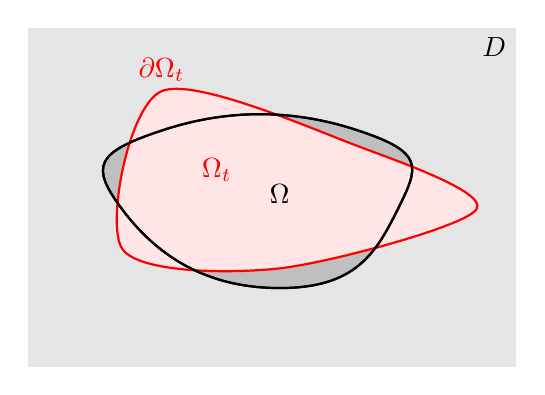
\begin{tikzpicture} [scale=1]
\fill[black!10] (-1.2,-2) rectangle (5,2.3);
\fill[black!25] plot[smooth cycle, tension = 1] coordinates {(0,0) (0.5,1) (3,1) (3.5,0) (2,-1)};
\fill[red!10] plot[smooth cycle] coordinates {(0,-0.5) (0.5,1.5) (3,0.8) (4.5,0) (2,-0.75)};
\draw[red, thick] plot[smooth cycle] coordinates {(0,-0.5) (0.5,1.5) (3,0.8) (4.5,0) (2,-0.75)};
\draw[thick] plot[smooth cycle, tension = 1] coordinates {(0,0) (0.5,1) (3,1) (3.5,0) (2,-1)};
\draw[thick] plot[smooth cycle, tension = 1] coordinates {(0,0) (0.5,1) (3,1) (3.5,0) (2,-1)};
\draw (2,0.2) node {$\Omega$};
\draw (5,2.3) node[below left] {$D$};
\draw[red] (0.5,1.5) node[above] {$\partial\Omega_t$};
\draw[red] (1.2,0.5) node {$\Omega_t$};
\end{tikzpicture}
\caption{A domain path}
\end{figure}

To apply gradient-based algorithms to the problem of optimizing over shape functions, a common approach is to introduce \textit{domain paths} $t\to\Omega_t$ and limits of the type
%
\begin{equation}
\frac d{dt}J_k(\Omega_t)\big|_{t=0}
%\lim_{t\to0^+}\frac{J_k(\Omega_t)-J_k(\Omega)}t
\end{equation}
%
in order to carry out a shape calculus in analogy to what is discussed in §\,\ref{s:Rn}.
Domain paths can be defined in various ways.
We will consider and compare two options: \textit{domain transformations} using perturbation of identity, and \textit{dilation of level-set boundaries}.

\section{Domain transformations}

A common way of creating domain paths is through a smooth vector field $\bs V\colon  D\to\RR^d$ and a transformation $T_{\bs V}:D\to\RR^d$ defined pointwise for each $\bs x\in D$ through the formula
%
\begin{equation}\label{e:TVdef}
T_{\bs V}(\bs x) = \bs x + \bs V(\bs x).
\end{equation}
%
Given transformation $T_{\bs V}$ and $\Omega\in\mathcal U$, we may define the shape derivative of a shape function $J$ as the directional derivative
%
\begin{equation}\label{e:dJtrans}
dJ(\Omega;\bs V) = \frac d{dt} J\bigl(T_{t\bs V}(\Omega)\bigr)\big|_{t=0}.      
\end{equation}
%
Shape function $J$ is said to be \textit{shape differentiable} if $dJ(\Omega; \bs V)$ exists for each $\bs V$ in a given Banach space and if $\bs V\mapsto dJ(\Omega;\bs V)$ is linear and continuous.

Similarly, we define the second shape derivative as 
%
\begin{equation}\label{e:d2Jtrans}
d^2 J(\Omega;\bs V, \bs W) = \frac{\partial^2}{\partial s\,\partial t} J\bigl(T_{t\bs V + s\bs W}(\Omega)\bigr)\big|_{t=s=0},
\end{equation}
%
and we say that $J$ is twice shape differentiable if $d^2J(\Omega; \bs V, \bs W)$ exists for each $\bs V$ and $\bs W$ in a given Banach space and if $(\bs V, \bs W)\mapsto d^2(\Omega; \bs V, \bs W)$ is bilinear and continuous.

With the help of these derivatives, we may, in analogy with definition~\eqref{e:mndef}, define the model function
%
\begin{equation}
M_n(\bs V) = dJ(\Omega; \bs V) + \frac12 dJ^2(\Omega; \bs V, \bs V),
\end{equation}
%
to be used in Newton’s method.

Derivatives~\eqref{e:dJtrans}, \eqref{e:d2Jtrans} are modeled after the last expressions in definitions~\eqref{e:gradient}, \eqref{e:Hessian}.
However, recall that in $\RR^n$, the Hessian can equivalently be defined as the derivative of the gradient vector $g$, as in the expression after the second equality in definition~\eqref{e:Hessian}.
Similarly, also here it is possible to define a second shape derivative as an iterated derivative,
%
\begin{equation}\label{e:ddJtrans}
dd J(\Omega; \bs V, \bs W) = \frac d{ds} dJ\bigl(T_{s\bs W}(\Omega);\bs V\bigr)\big|_{s=0}.
\end{equation}
%
However, in this case, the second derivatives~\eqref{e:d2Jtrans} and \eqref{e:ddJtrans} are not the same in general.
The reason is that for definition~\eqref{e:Hessian}, the unit vectors $e_i$, $e_j$ are constant, whereas the displacement vector $\bs V$ in definition~\eqref{e:TVdef} is not.
Indeed, let $T_{t\bs V}(\bs x) = \bs x + t\bs V(\bs x) = \hat{\bs x}$ and consider the iterated transformation that satisfies
%
\begin{equation}\label{e:TsWTtV}
\begin{aligned}
T_{s\bs W}\bigl(T_{t\bs V}(\bs x)\bigr) &= T_{s\bs W}(\hat{\bs x}) 
=\hat{\bs x} + s\bs W(\hat{\bs x}) 
\\
&= \bs x + t\bs V(\bs x) + s\bs W\bigl(\bs x + t\bs V(\bs x)\bigr), 
\end{aligned}
\end{equation}
%
from which we can conclude that $T_{s\bs W}\bigl(T_{t\bs V}(\bs x)\bigr) = \bs x + t\bs V(\bs x) + s\bs W(\bs x)$ is only guaranteed to hold if $\bs W$ is a constant vector field.  

The second derivative mapping $(\bs V, \bs W) \mapsto d^2J(\Omega; \bs V, \bs W)$ is symmetric due to the commutativity of ordinary addition, whereas expression~\eqref{e:TsWTtV} shows that $(\bs V, \bs W) \mapsto ddJ(\Omega; \bs V, \bs W)$ is not.
However $ddJ$ has the advantage to be easy to compute by iterating known shape calculus expressions.
Fortunately, $d^2J$ can be computed from $dd J$ using the following property.
%
\begin{theorem}
Consider mapping $T_{\bs V}:D\to\RR^d$ defined pointwise as in expression~\eqref{e:TVdef}.
Given vector fields $\bs V, \bs W$ on $D$, assume that mapping $T_{s\bs W}$ is a homeomorphism for $s$ in the vicinity of 0. 
Then 
%
\begin{equation}
d^2 J(\Omega; \bs V, \bs W) = dd J(\Omega; \bs V, \bs W) - dJ\bigl(\Omega;(\bs W\cdot\nabla)\bs V \bigr)
\end{equation}
%
\textcolor{red}{[will need more specifications of $\bs V, \bs W$, $\Omega$, $J$]}
\end{theorem}
%
\begin{proof}
Given vector fields $\bs V$ and $\bs W$, define $\bs Z = \bs V\circ T_{s\bs W}^{-1}$, which is well defined for $s$ in the vicinity of 0, from which it follows that
%
\begin{equation}\label{e:ZT}
\bs V = \bs Z\circ T_{s\bs W}.    
\end{equation}
%
Moreover, for any $\bs x\in D$,
%
\begin{equation}
\begin{aligned}
\bs Z(\bs x) &= \bigl(\bs V\circ T_{s\bs W}^{-1}\bigr)(\bs x)
= \bs V\bigl((\bs x + s\bs W(\bs x)^{-1}\bigr)
= \bs V\bigl(\bs x - s\bs W((\bs x) + o(s)\bigr)
\\
&= \bs V(\bs x) -s\bs W(\bs x)\cdot\nabla\bs V(\bs x) + o(s),
\end{aligned}
\end{equation}
%
where Taylor expansions have been used in the third and fourth equality.

With the help of these preliminary steps, we consider
%
\begin{equation}\label{e:TtVsW}
\begin{aligned}
T_{t\bs V + s\bs W}(\bs x) &= \bs x + t\bs V(\bs x) + s\bs W(\bs x)
= \bs x + s\bs W(\bs x) + t(\bs Z\circ T_{s\bs W})(\bs x) 
\\
&= T_{s\bs W}(\bs x) + t(\bs Z\circ T_{s\bs W})(\bs x) 
= (T_{t\bs Z}\circ T_{s\bs W})(\bs x),
\end{aligned}
\end{equation}
%
where expression~\eqref{e:ZT} is used in the second equality.
%
From equality~\eqref{e:TtVsW} follows that
%
\begin{equation}
\begin{aligned}
\frac\partial{\partial t} J\bigl(T_{t\bs V + s\bs W}(\Omega)\bigr)\big|_{t=0}
&= \frac\partial{\partial t} J\bigl((T_{t\bs Z}\circ T_{s\bs W})(\Omega)\bigr)\big|_{t=0}
= dJ\bigl(T_{s\bs W}(\Omega);\bs Z\bigr)
\\
&=dJ\bigl(T_{s\bs W}(\Omega);\bs V\bigr)-
s\,dJ\bigl(T_{s\bs W}(\Omega);\bs W\cdot\nabla\bs V\bigr) + o(s).
\end{aligned}    
\end{equation}

\end{proof}


\end{document}
